% ============================================================
% f2014_beijing_science_q17_pyramid.tex
% 2014 北京卷（理科）第 17 题：五棱锥 P-ABCDE
% 来源 PDF：普通高考/2014/2014北京理.pdf
% 原页：第 1 页（A3），印面 861，右栏第 17 题题干下方
% 底面为正方形 AMDE（边长 2）截去 △MBC，B、C 分别为 AM、MD 中点；
% F 为 PE 中点，截面 ABF 与 PD、PC 交于 G、H，截面为五边形 ABHGF。
% 斜二测投影：px = X + 0.52Y，py = Z + 0.62Y（再乘 1.6 作尺寸）。
% ============================================================
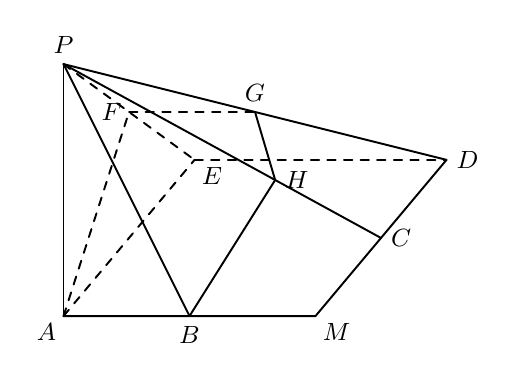
\begin{tikzpicture}[line width=0.7pt, font=\small,
  line cap=round, line join=round]
  % 顶点（斜二测投影后的纸面坐标）
  \coordinate (P)  at (0,3.200);
  \coordinate (A)  at (0,0);
  \coordinate (B)  at (1.600,0);
  \coordinate (M)  at (3.200,0);
  \coordinate (C)  at (4.032,0.992);
  \coordinate (D)  at (4.864,1.984);
  \coordinate (E)  at (1.664,1.984);
  \coordinate (F)  at (0.832,2.592);  % PE 中点
  \coordinate (G)  at (2.432,2.592);  % PD 中点
  \coordinate (H)  at (2.688,1.728);  % PC 上，PH:HC=2:1

  % 被遮挡的棱与截面边
  \draw[dashed] (P) -- (E);
  \draw[dashed] (A) -- (E);
  \draw[dashed] (E) -- (D);
  \draw[dashed] (A) -- (F);
  \draw[dashed] (F) -- (G);

  % 可见的棱
  \draw (P) -- (A);
  \draw (P) -- (B);
  \draw (P) -- (C);
  \draw (P) -- (D);
  \draw (A) -- (B) -- (M) -- (C) -- (D);

  % 可见的截面边
  \draw (B) -- (H) -- (G);

  % 标注
  \node[above] at (P) {$P$};
  \node[left=-1pt] at (F) {$F$};
  \node[above] at (G) {$G$};
  \node[right] at (H) {$H$};
  \node[below right=-1pt] at (E) {$E$};
  \node[below left=-1pt] at (A) {$A$};
  \node[below] at (B) {$B$};
  \node[below right=-1pt] at (M) {$M$};
  \node[right] at (C) {$C$};
  \node[right] at (D) {$D$};
\end{tikzpicture}
